\documentclass[aspectratio=43]{beamer}
\usepackage[utf8]{inputenc}
\usepackage[T1]{fontenc}

% Chinese
\usepackage{xeCJK}
\usepackage{fontspec} 
\setCJKmainfont{SimSun} %或\setCJKmainfont{KaiTi}
\setCJKmonofont{SimSun}
\setmainfont{Times New Roman}

% Figures
\usepackage{graphicx,times}
\usepackage{subfigure}         

\usepackage{geometry}
\geometry{left=0.5cm,right=0.5cm,top=0cm,bottom=0cm}


%==========citation===========
\usepackage{url}

\title{红外高光谱数据压缩与评估}
\date{\today}
\author[Feng]{Mia Feng}

\usetheme{material}

\useLightTheme
\usePrimary{4527A0}{311B92}{FFFFFF}
\useAccent{C6FF00}{000000}


\begin{document}

\begin{frame}
\titlepage
\end{frame}

\section{Before}
\begin{frame}{云检测:logistic,random forest}
仅重述前几次听报告的一些思考。
\begin{cardTiny}
分类问题解决方法:
\begin{itemize}
\item 分类平面:几何距离(SVM)、概率分布(logistic)。
\item 分类规则:decision tree (DT), random forest (RF)。
\end{itemize}
\end{cardTiny}
\centering
\cardImg{img/concept/ML--MAP.png}{0.8\textwidth}
\begin{cardTiny}
Logistic:loss选择的是交叉熵,参数估计方法是最大似然。\\
RF,DT: loss选择的是互信息(信息容量)或者其改进版。\\
3DVAR、4DVAR:最大化后验,可视为{\color{green}生成式模型?}
\end{cardTiny}
\end{frame}


\section{catalogue}
\begin{frame}
\begin{card}[目录]
\begin{itemize}
\item 红外高光谱数据的特点
\item 红外高光谱数据压缩方法
\item 基于KPCA的红外高光谱数据压缩
\item 高光谱数据压缩评估指标
\item 问题
\end{itemize}
%\\\url{https://material.io}
\end{card}
\end{frame}


\section{Sec1}
\begin{frame}{数据特点}
\begin{card}
\textbf{高空间相关性} \\[2mm]
每个谱带内某一像素与其{\color{primary}相邻像素}之间的相似性
\end{card}
\begin{card}
\textbf{高谱间相关性}\\ [2mm]
{\color{primary}不同谱带}的图像在同一空间位置的像素具有相似性
\end{card}
\begin{card}
\textbf{稀疏性}\\ [2mm]
高光谱数据的高维空间大部分都是空的。
\end{card}
\end{frame}

\begin{frame}{空间相关性}
\begin{card}[图像自相关函数]
%\begin{equation}
%r\left(l,k\right)=\frac{\sum\limits_{x=1}^{M}\sum\limits_{y=1}^{N}\left(f\left(x,y\right)-u_f\right)*\left(f\left(x+l,y+k\right)-u_f\right)}{\sum\limits_{x=1}^{M}\sum\limits_{y=1}^{N}\left(f\left(x,y\right)-u_f\right)^2}
%\end{equation}
\begin{equation}
r_x\left(l\right)=\frac{\sum\limits_{x=1}^{M}\sum\limits_{y=1}^{N}\left(f\left(x,y\right)-u_f\right)*\left(f\left(x+l,y\right)-u_f\right)}{\sum\limits_{x=1}^{M}\sum\limits_{y=1}^{N}\left(f\left(x,y\right)-u_f\right)^2}
\end{equation}
\begin{equation}
r_y\left(k\right)=\frac{\sum\limits_{x=1}^{M}\sum\limits_{y=1}^{N}\left(f\left(x,y\right)-u_f\right)*\left(f\left(x,y+k\right)-u_f\right)}{\sum\limits_{x=1}^{M}\sum\limits_{y=1}^{N}\left(f\left(x,y\right)-u_f\right)^2}
\end{equation}
\end{card}
\end{frame}

\begin{frame}{空间相关性}
\begin{card}[自相关系数]
\begin{equation}
\rho_x=\frac{\sum\limits_{x=1}^{M}\sum\limits_{y=1}^{N}\left(f\left(x,y\right)-u_f\right)*\left(f\left(x+1,y\right)-u_f\right)}{\sum\limits_{x=1}^{M}\sum\limits_{y=1}^{N}\left(f\left(x,y\right)-u_f\right)^2} 
\end{equation}
\begin{equation}
\rho_y=\frac{\sum\limits_{x=1}^{M}\sum\limits_{y=1}^{N}\left(f\left(x,y\right)-u_f\right)*\left(f\left(x,y+1\right)-u_f\right)}{\sum\limits_{x=1}^{M}\sum\limits_{y=1}^{N}\left(f\left(x,y\right)-u_f\right)^2}
\end{equation}
\end{card}
\end{frame}

\begin{frame}{空间相关性}
\begin{figure}
  \centering
  \subfigure[行自相关系数]{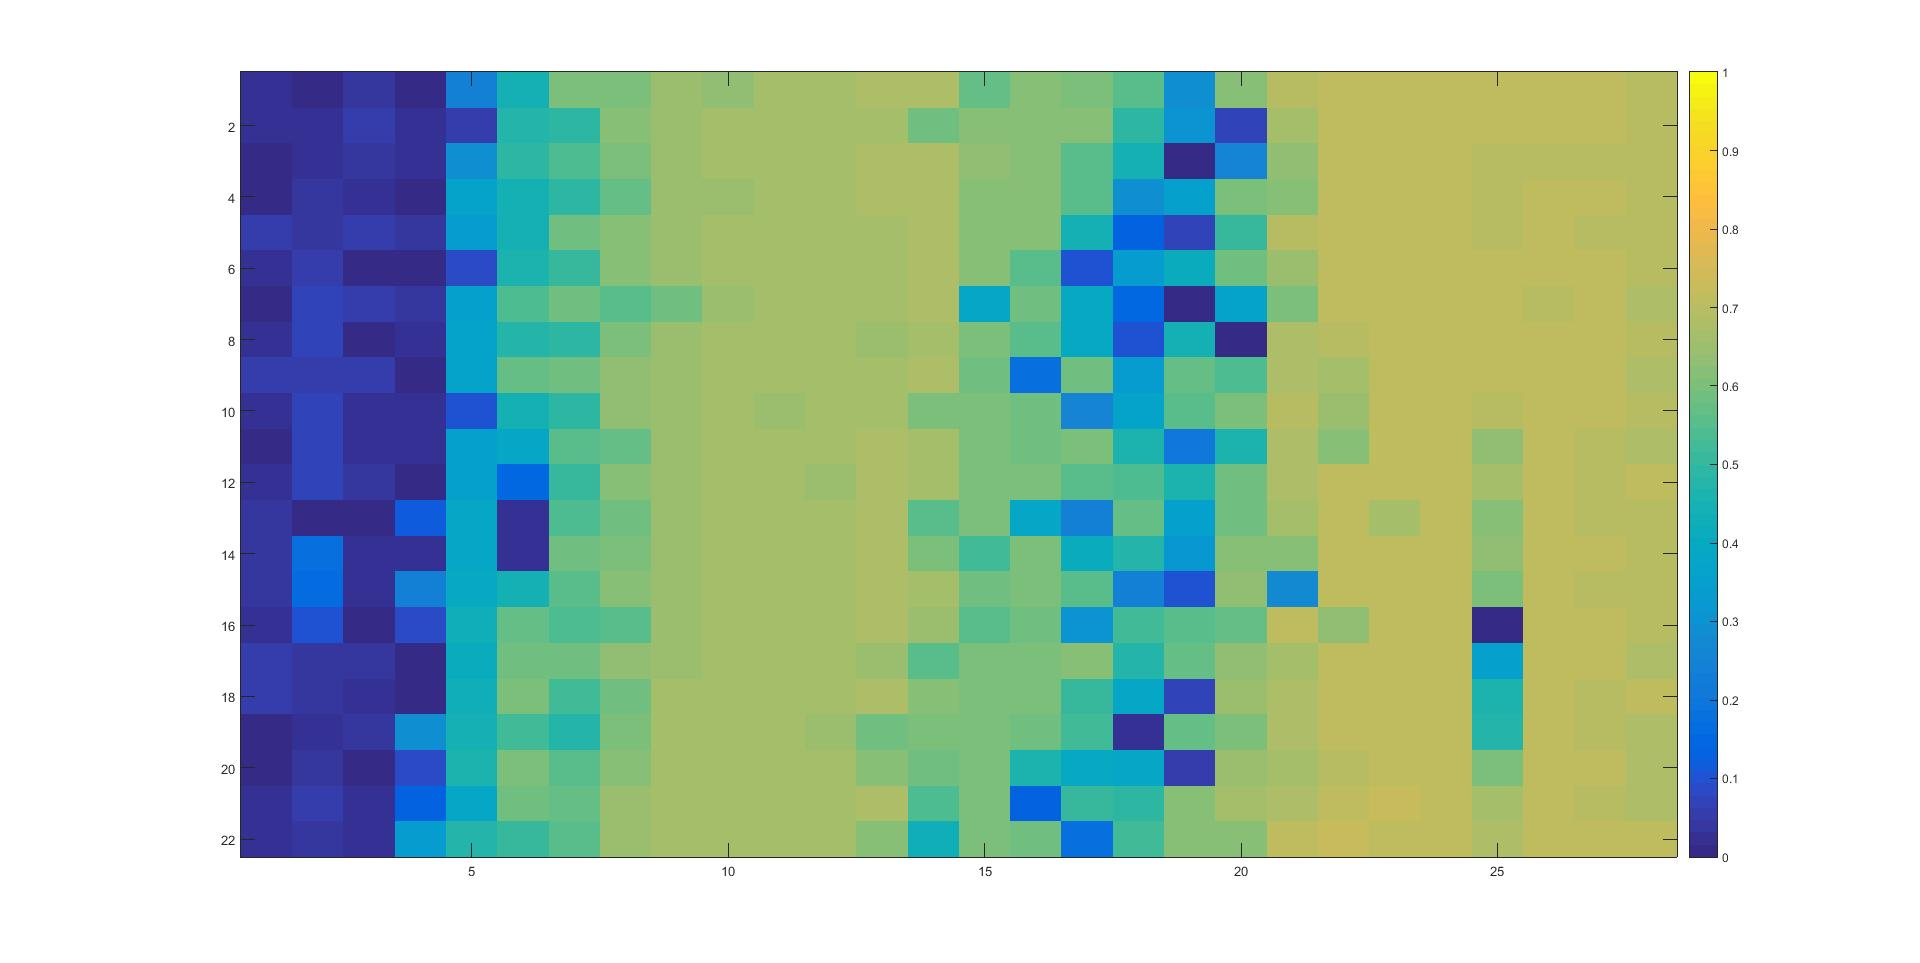
\includegraphics[width=2in]{img/corr_coeff/spatial_row_corr.jpg}}
  \subfigure[列自相关系数]{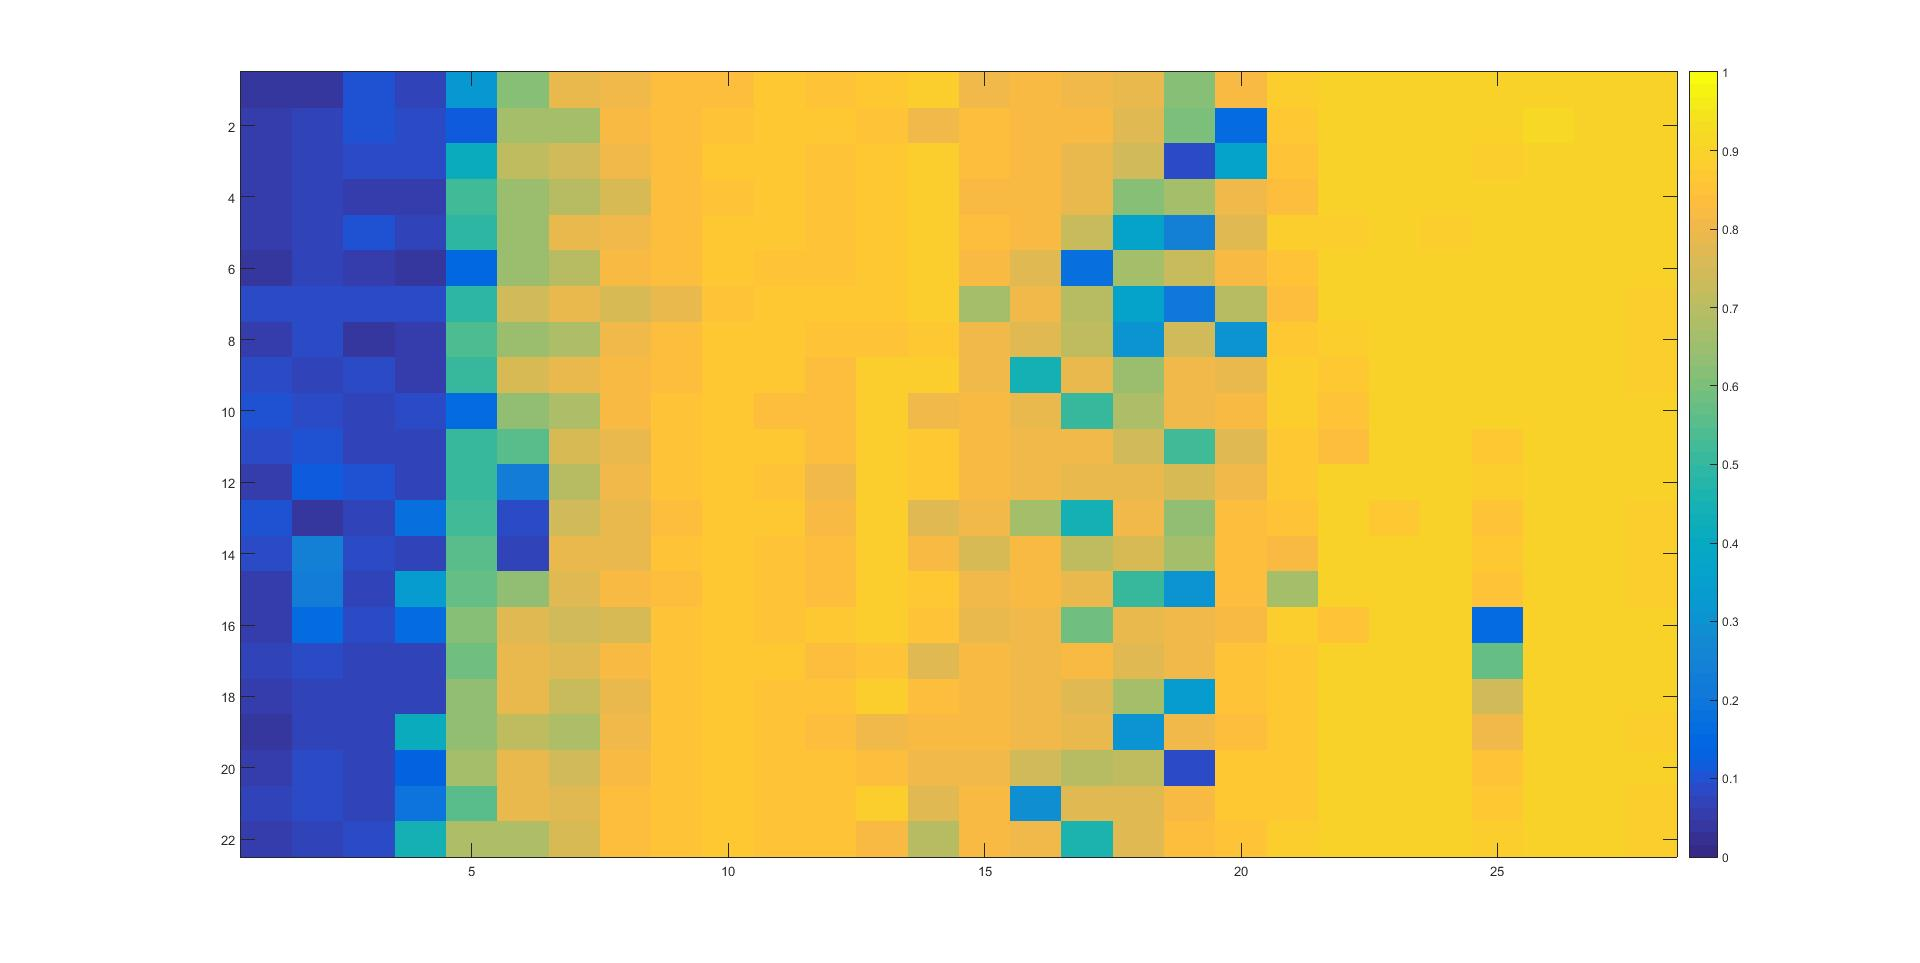
\includegraphics[width=2in]{img/corr_coeff/spatial_col_corr.jpg}}
  \caption{ 自相关系数 }
\end{figure}
\end{frame}

\begin{frame}{谱间相关性}
\begin{card}
\begin{equation}
h\left(l,k\right)=\frac{\sum\limits_{x=1}^{M}\sum\limits_{y=1}^{N}\left(f\left(x,y\right)-u_f\right)*\left(g\left(x+l,y+k\right)-u_g\right)}{\sqrt{\left(\sum\limits_{x=1}^{M}\sum\limits_{y=1}^{N}\left(f\left(x,y\right)-u_f\right)^2\right)\left(\sum\limits_{x=1}^{M}\sum\limits_{y=1}^{N}\left(g\left(x,y\right)-u_g\right)^2\right)}}
\end{equation}
\begin{equation}
h_{i,j}=\frac{\sum\limits_{x=1}^{M}\sum\limits_{y=1}^{N}\left(f\left(x,y\right)-u_f\right)*\left(g\left(x,y\right)-u_g\right)}{\sqrt{\left(\sum\limits_{x=1}^{M}\sum\limits_{y=1}^{N}\left(f\left(x,y\right)-u_f\right)^2\right)\left(\sum\limits_{x=1}^{M}\sum\limits_{y=1}^{N}\left(g\left(x,y\right)-u_g\right)^2\right)}}
\end{equation}
\end{card}
\end{frame}

\begin{frame}{谱间相关性}
\begin{card}
\begin{equation}
h_{i}=\frac{\sum\limits_{x=1}^{M}\sum\limits_{y=1}^{N}\left(f_i\left(x,y\right)-u_i\right)*\left(f_{i}\left(x,y\right)-u_{i}\right)}{\sqrt{\left(\sum\limits_{x=1}^{M}\sum\limits_{y=1}^{N}\left(f_i\left(x,y\right)-u_i\right)^2\right)\left(\sum\limits_{x=1}^{M}\sum\limits_{y=1}^{N}\left(f_{i+1}\left(x,y\right)-u_{i+1}\right)^2\right)}}
\end{equation}
\end{card}
\end{frame}


\begin{frame}{谱间相关性}
\begin{figure}
  \centering
\cardImg{img/corr_coeff/spectrum_corr.jpg}{0.8\textwidth}{不同谱带间的自相关系数}

\end{figure}
{\color{primary}谱间相关性强于空间相关性。}
\end{frame}

\begin{frame}{稀疏性}
\begin{card}
高光谱数据的高维空间大部分都是空的,所以可以用低维空间去近似表示高维空间,而不会带来较大的误差。
推导证明见page 19-21\cite{陈雨时2014}。

以IASI为例,光谱通道计8461个,进入同化的通道计616个。
\end{card}
\begin{card}[The curse of dimensionality]
通常是指在涉及到向量的计算的问题中,随着维数的增加,计算量呈指数倍增长的一种现象。它描述的是当(数学)空间维度增加时,分析和组织高维空间(通常有成百上千维)中的数据,因{\color{primary}体积指数增加}而遇到各种问题场景。
%也解释了为什么随着特征维数的增加,所需要的数据要更多,因为数据密度不够。在DNNs时,所需要的数据量更多。
\end{card}
\end{frame}



\section{Reduction}
\begin{frame}{降维方法}
\begin{itemize}
\item 波段选择:特征子空间。
\item 特征提取:坐标变换。
\item 混合方法:波段选择+特征提取。
\end{itemize}
\begin{card}
采用这些降维方法,构建回归方程或者设计码书({\color{green}可以看做离散型的映射和连续型的映射?}),可以完成对红外高光谱数据的压缩。
\end{card}
\end{frame}

\section{Compression}
\begin{frame}{基于预测的压缩技术}
\begin{card}
一个谱带可以由相邻的谱带预测,其产生的去相关之后的残余误差比较容易压缩。
\end{card}
\begin{card}[步骤]
\begin{itemize}
\item 选取参考谱带:查找准则(等间隔、BH距离、JM距离等);查找算法(最优与次优,SFS、SBS,SFFS、SBFS)
\item 建立回归方程:单、双向(是否利用预测的谱带建立回归方程);多元线性回归。{\color{green}??}
\end{itemize}
\end{card}
\end{frame}

\begin{frame}{基于矢量量化的压缩技术}
\begin{card}[Idea]
{\color{primary}编码}(码书设计)和{\color{primary}解码}(码字搜索),分为{\color{primary}基于特征选择}的矢量量化技术和{\color{primary}基于特征变换}的矢量量化技术。\\  [2mm]
以PCA为例,编码利用特征向量,解码利用特征向量的逆。也可选择一些子波段用来进行编码(利用高通道冗余性)\cite{Pellet2016Dimension}。
%解码利用特征向量的逆( 或者转置 when they are orthogonal )。%
\end{card}
%
%\begin{card}
%{\color{primary} \textbackslash begin\{card\}[Title]\\[2mm]}
%\null\qquad \textit{[your content here]}\\[2mm]
%{\color{primary} \textbackslash end\{card\}}
%\end{card}
\end{frame}

\section{KPCA}
\begin{frame}{基于KPCA的红外高光谱数据压缩}
\begin{card}
与PCA的不同:核方法完成非线性映射,可以处理非高斯分布的原始数据。\\
优点:提取非线性映射特征。\\
缺点:重构的非线性映射算子无法显式得到,需要迭代近似,计算量。且为了迭代近似,需要压缩前的数据。
\end{card}
\begin{cardTiny}[步骤]
\begin{itemize}
\item 核矩阵计算(非线性映射):{\color{green}核函数的选择}。
\item 计算特征向量,并按特征值大小排序。\\{\color{primary}Hint:为什么PCA中top k个特征向量重构出的损失最小,证明参见 section 2.12\cite{Goodfellow2016Deep}。}
\item 重构。可以在重构时,对不同PC成分指定不同的权重系数。从而分析不同的PC可能提取了哪些特征。
\end{itemize}
\end{cardTiny}
\end{frame}


\begin{frame}{重构结果\cite{Wang2012Kernel,Mika1999Kernel}}
\centering
\cardImg{img/pc_fea_mean/Origin.jpg}{0.5\textwidth}
原数据:51(纬度)*120(经度)*616(通道数)\\
空间上平均后的结果:每个格点代表一个通道在51*120上的平均结果\\
{\color{green}这些图展示的结果没有意义,但我目前只有这些数据。所以这里只说明分析思路。}
\end{frame}

\begin{frame}{重构结果——各PC在重构中给定权重不同时的结果}
\begin{figure}
  \centering
  \subfigure[PC 1]{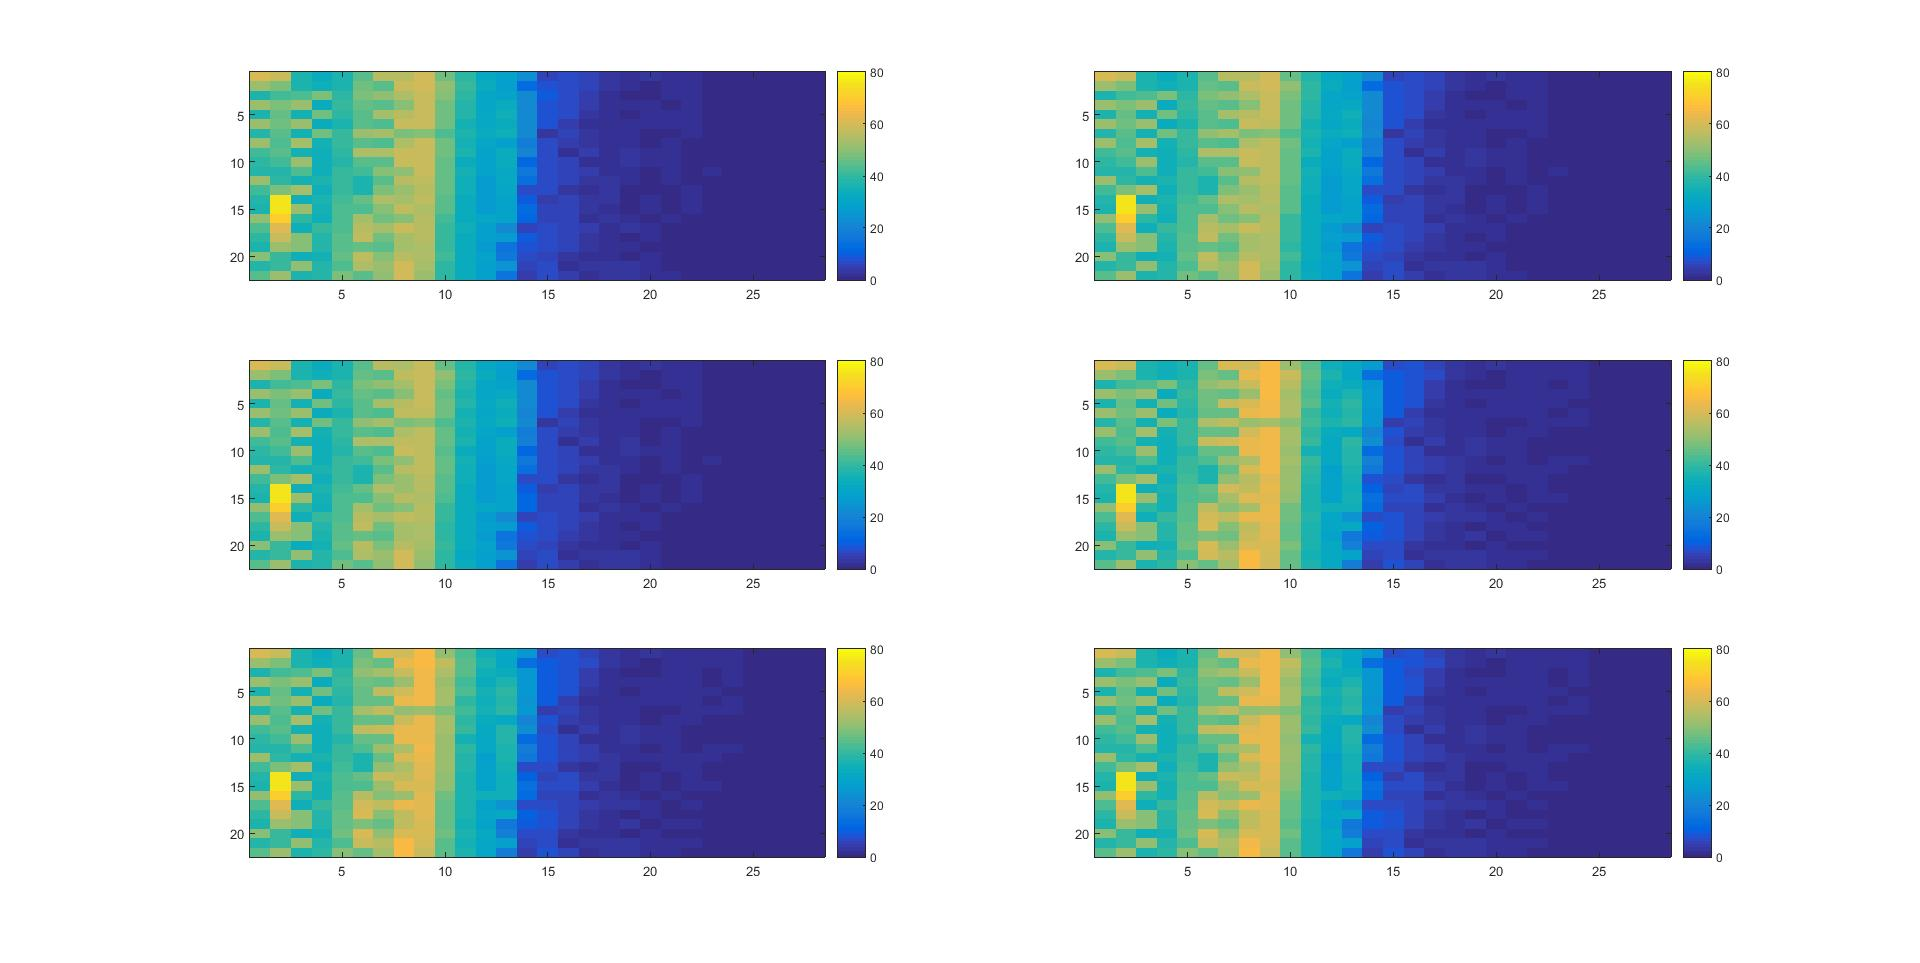
\includegraphics[width=2in]{img/pc_fea_mean/PC1.jpg}}
  \subfigure[PC 2]{\includegraphics[width=2in]{img/pc_fea_mean/PC2.jpg}}
  \caption{PC重构敏感性}
\end{figure}
\end{frame}

\begin{frame}{重构结果——各PC在重构中给定权重不同时的结果}
\begin{figure}
  \centering
  \subfigure[PC 3]{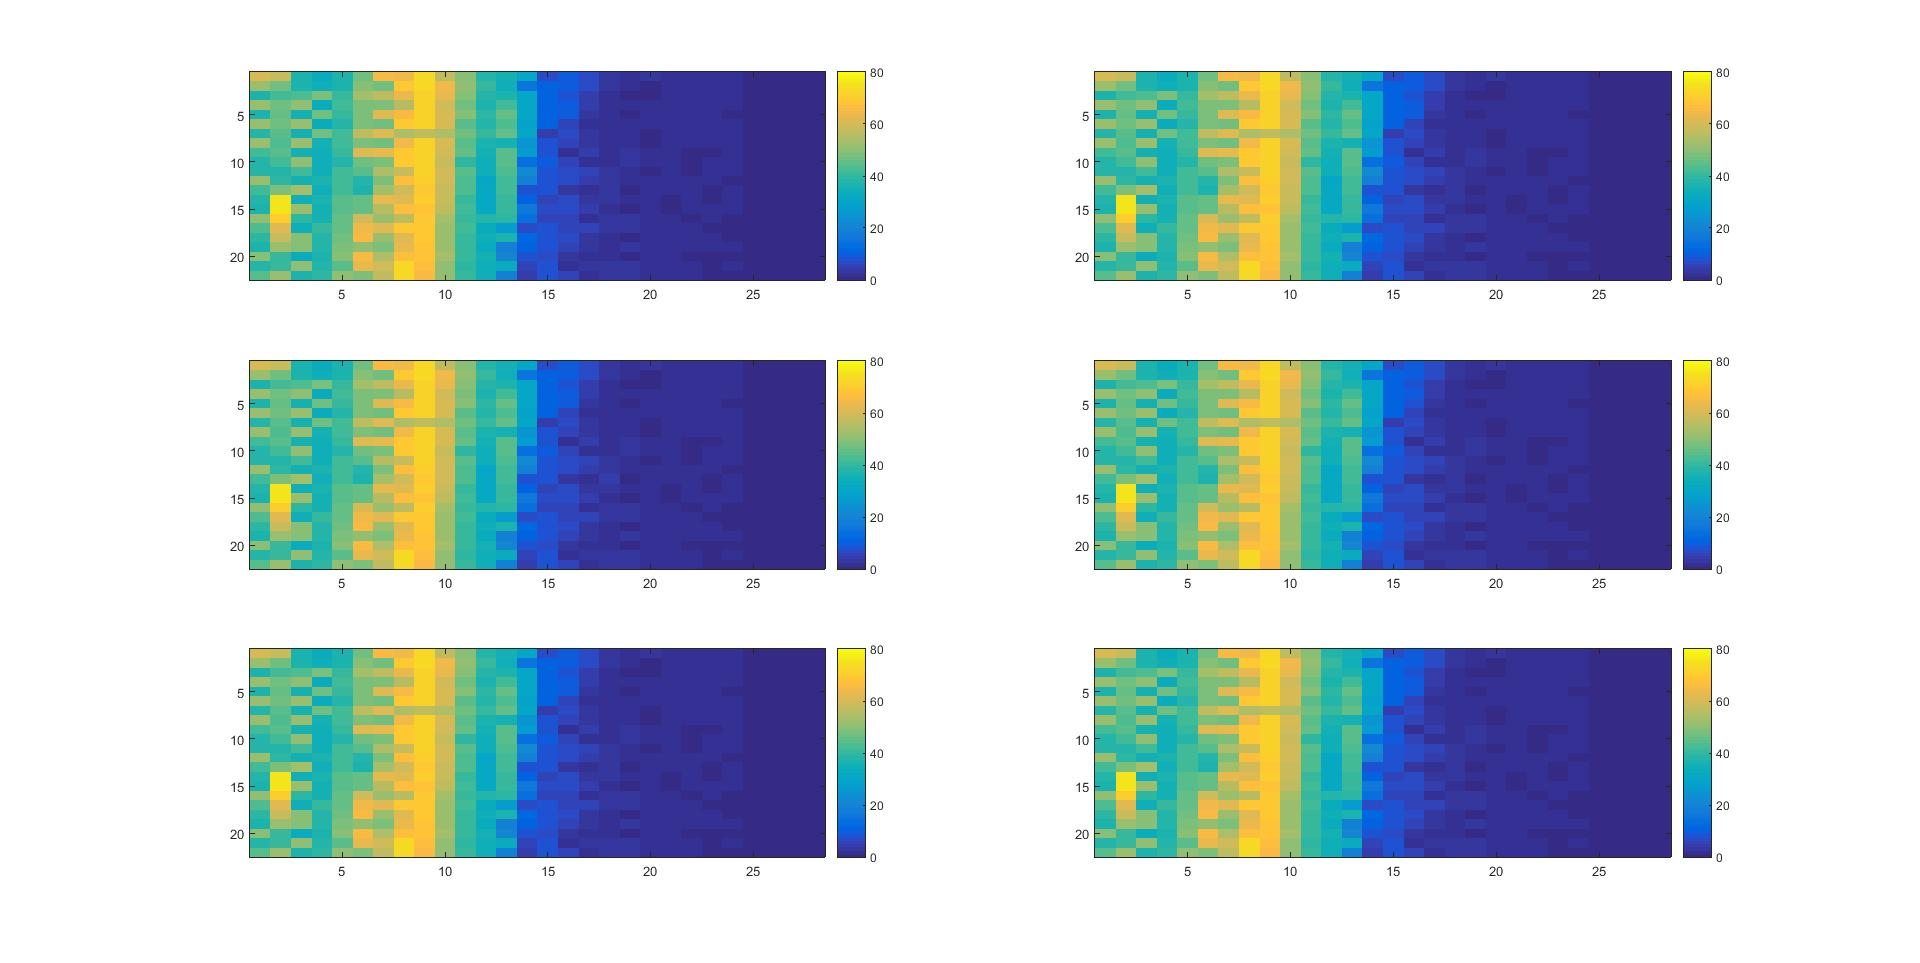
\includegraphics[width=2in]{img/pc_fea_mean/PC3.jpg}}
  \subfigure[PC 4]{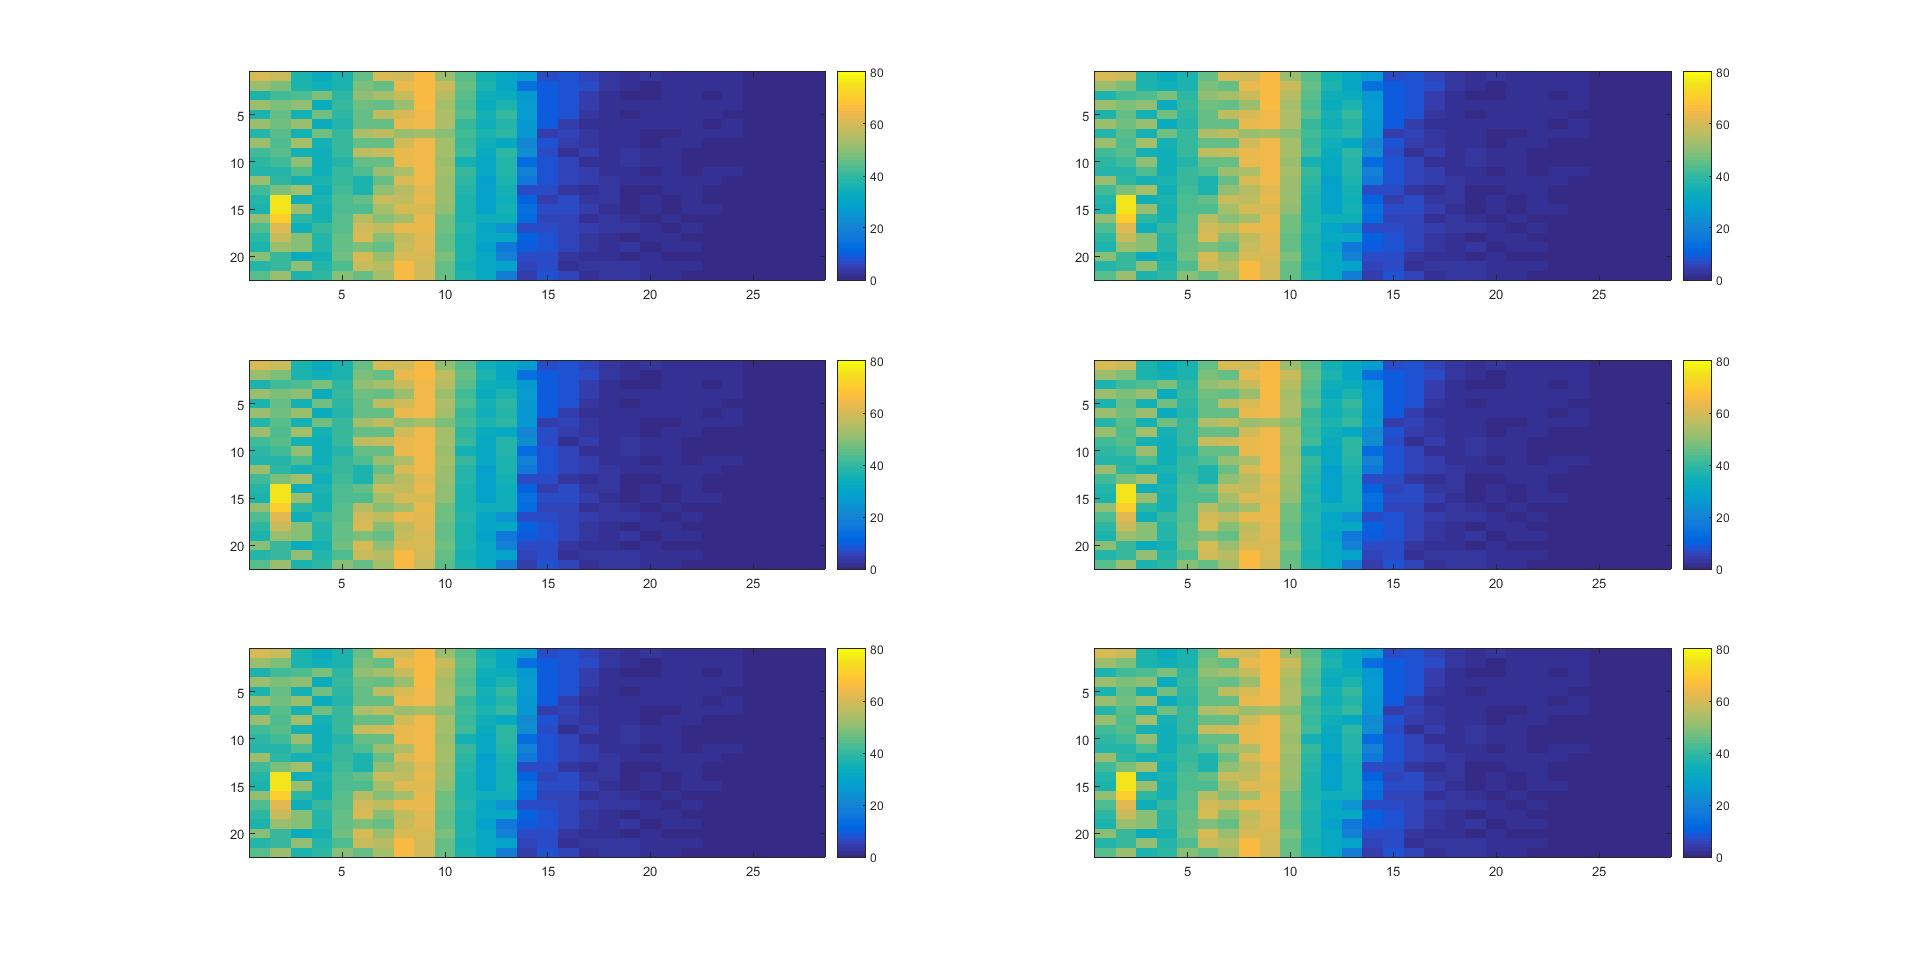
\includegraphics[width=2in]{img/pc_fea_mean/PC4.jpg}}
  \caption{ PC重构敏感性 }
\end{figure}
\end{frame}

\begin{frame}{重构结果——各PC在重构中给定权重不同时的结果}
\begin{figure}
  \centering
  \subfigure[PC 5]{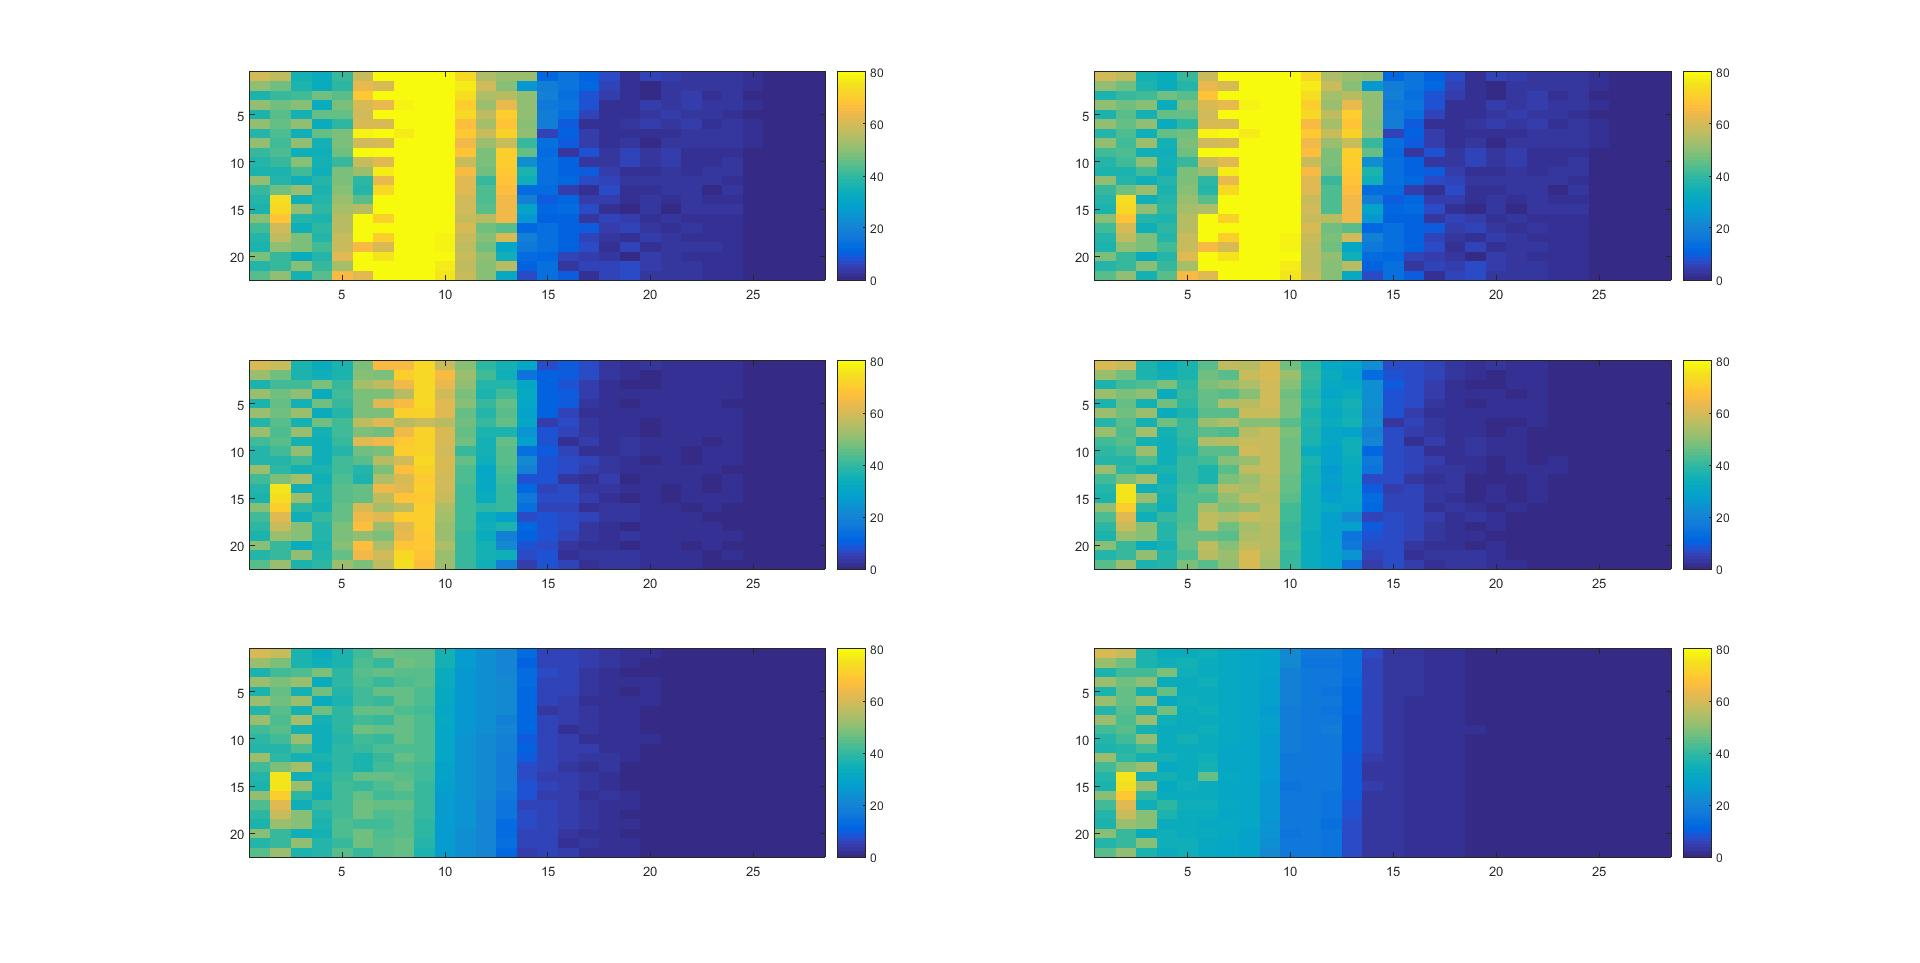
\includegraphics[width=2in]{img/pc_fea_mean/PC5.jpg}}
  \subfigure[PC 6]{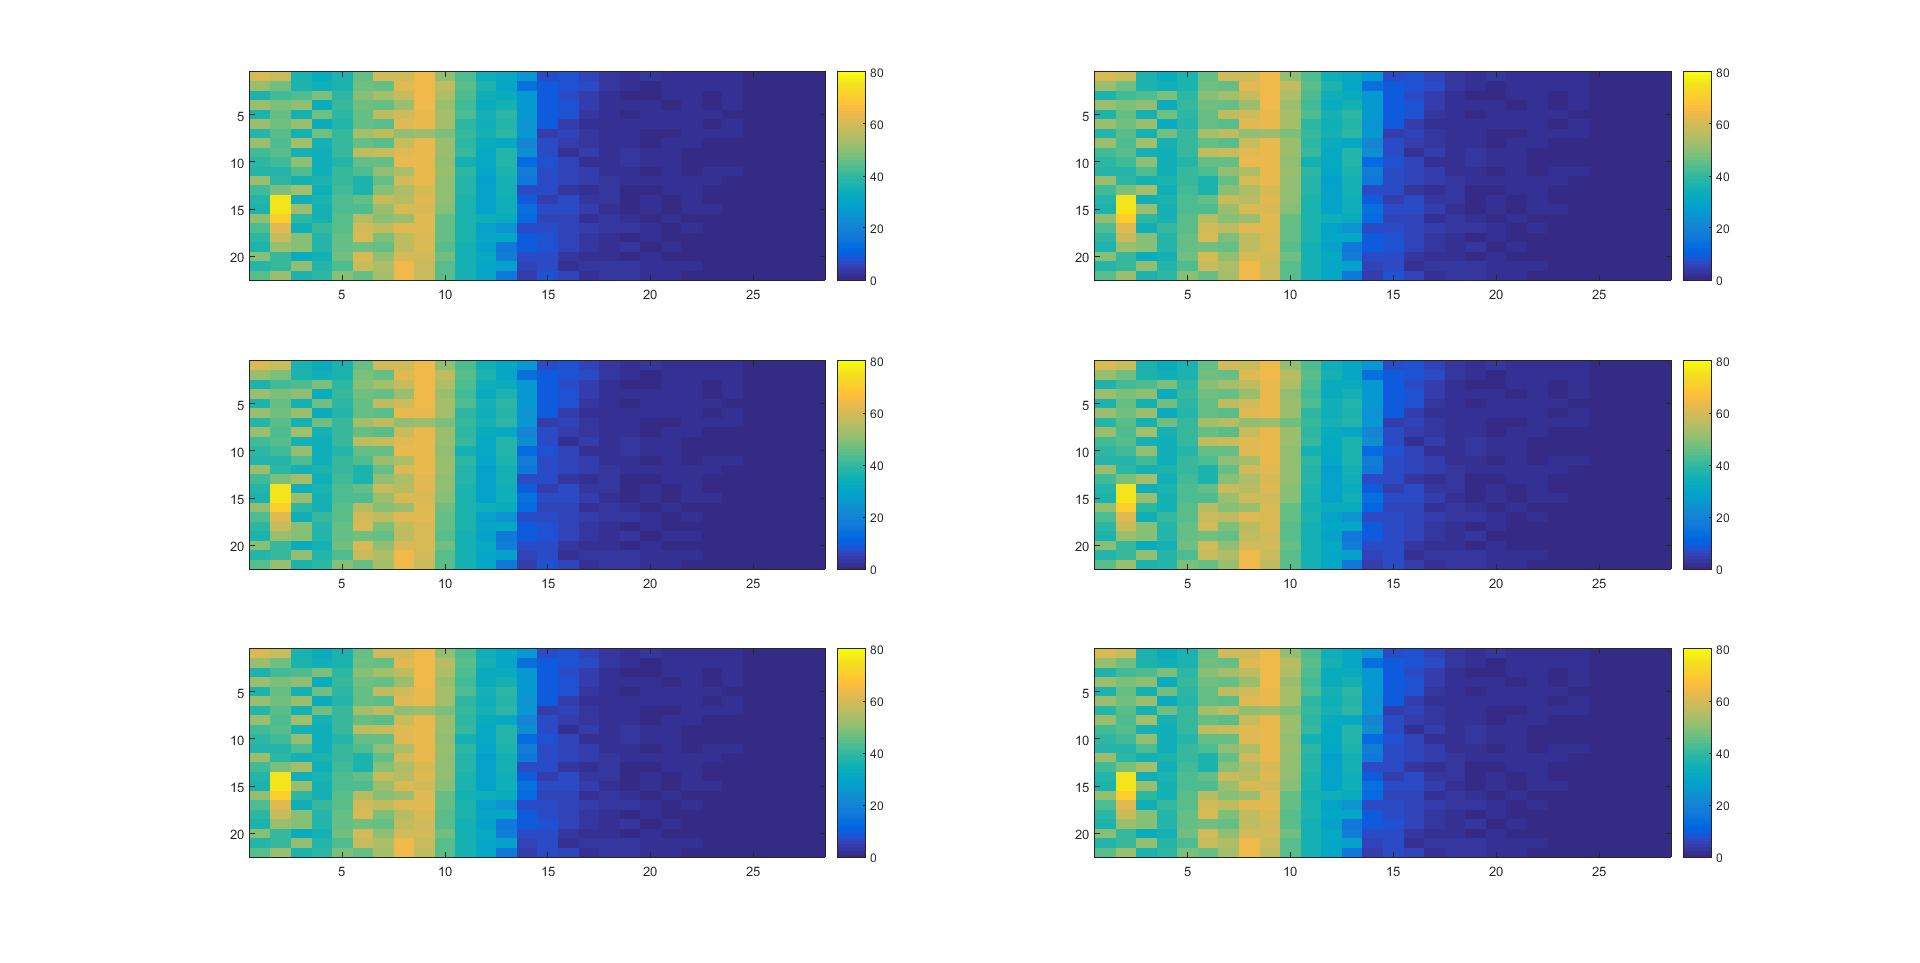
\includegraphics[width=2in]{img/pc_fea_mean/PC6.jpg}}
  \caption{ PC重构敏感性 }
\end{figure}
\end{frame}

\begin{frame}{重构结果——各PC在重构中给定权重不同时的结果}
\begin{figure}
  \centering
  \subfigure[PC 7]{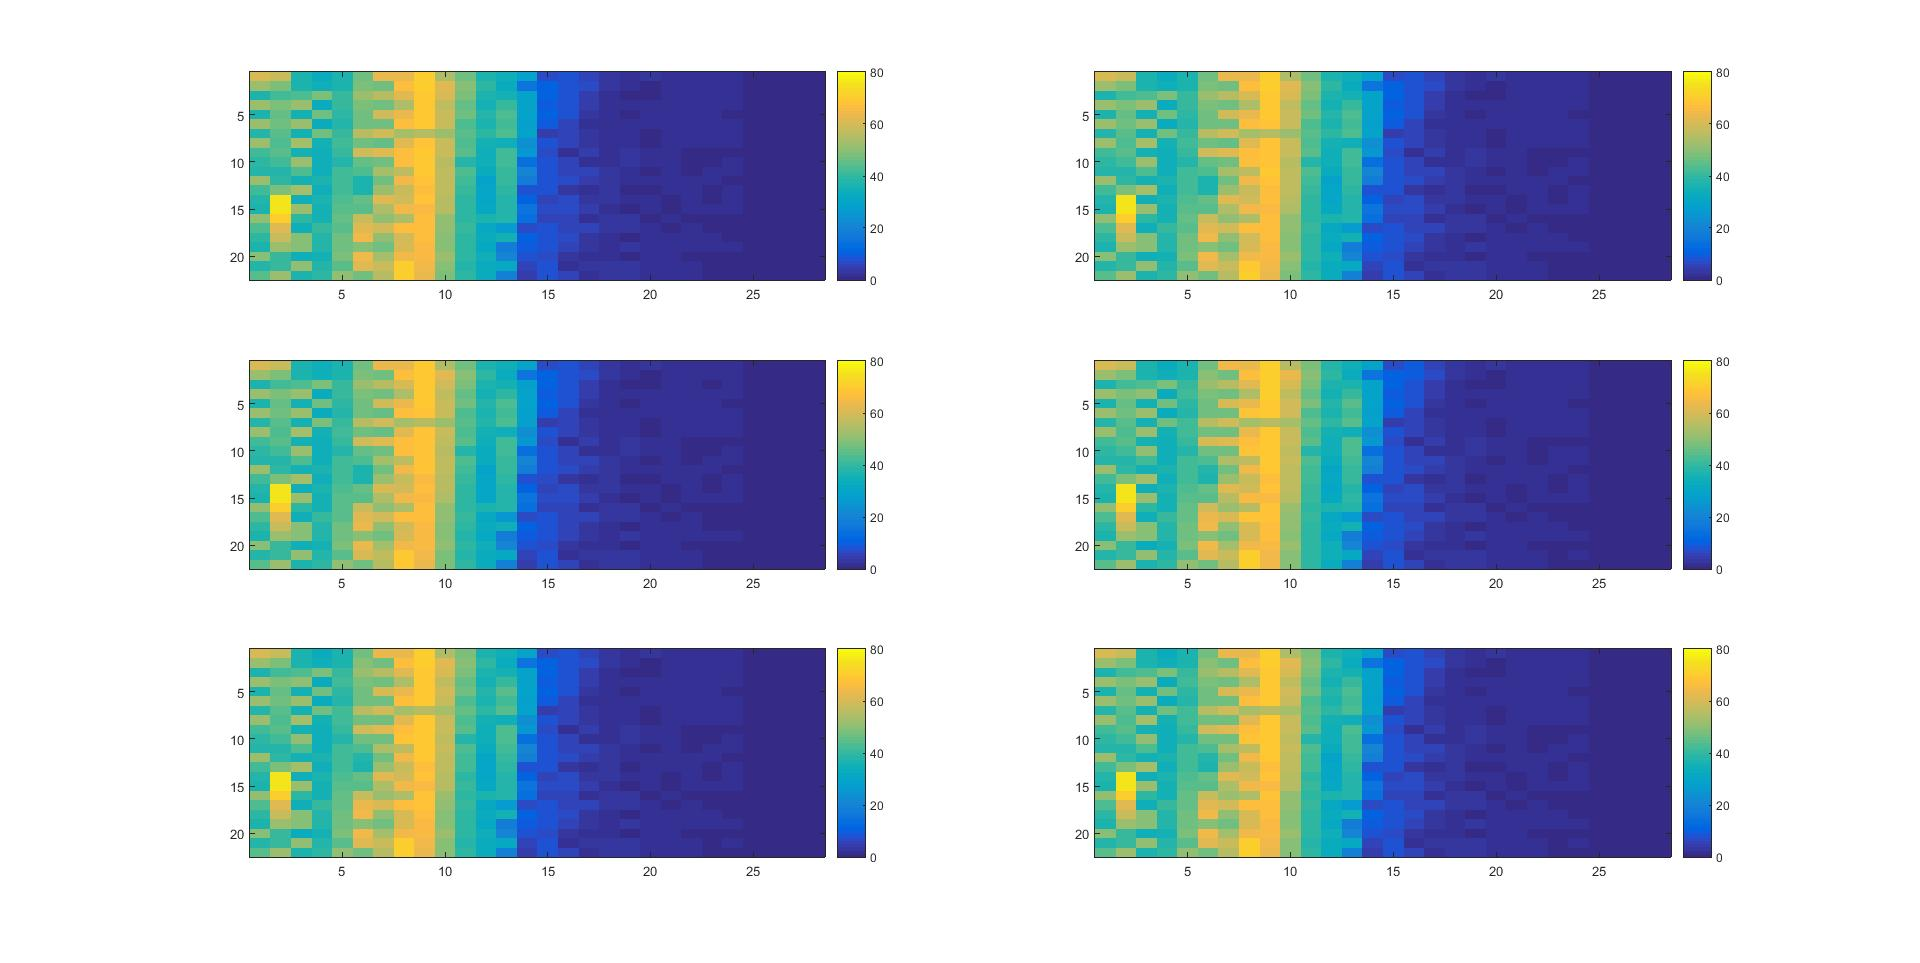
\includegraphics[width=2in]{img/pc_fea_mean/PC7.jpg}}
  \subfigure[PC 8]{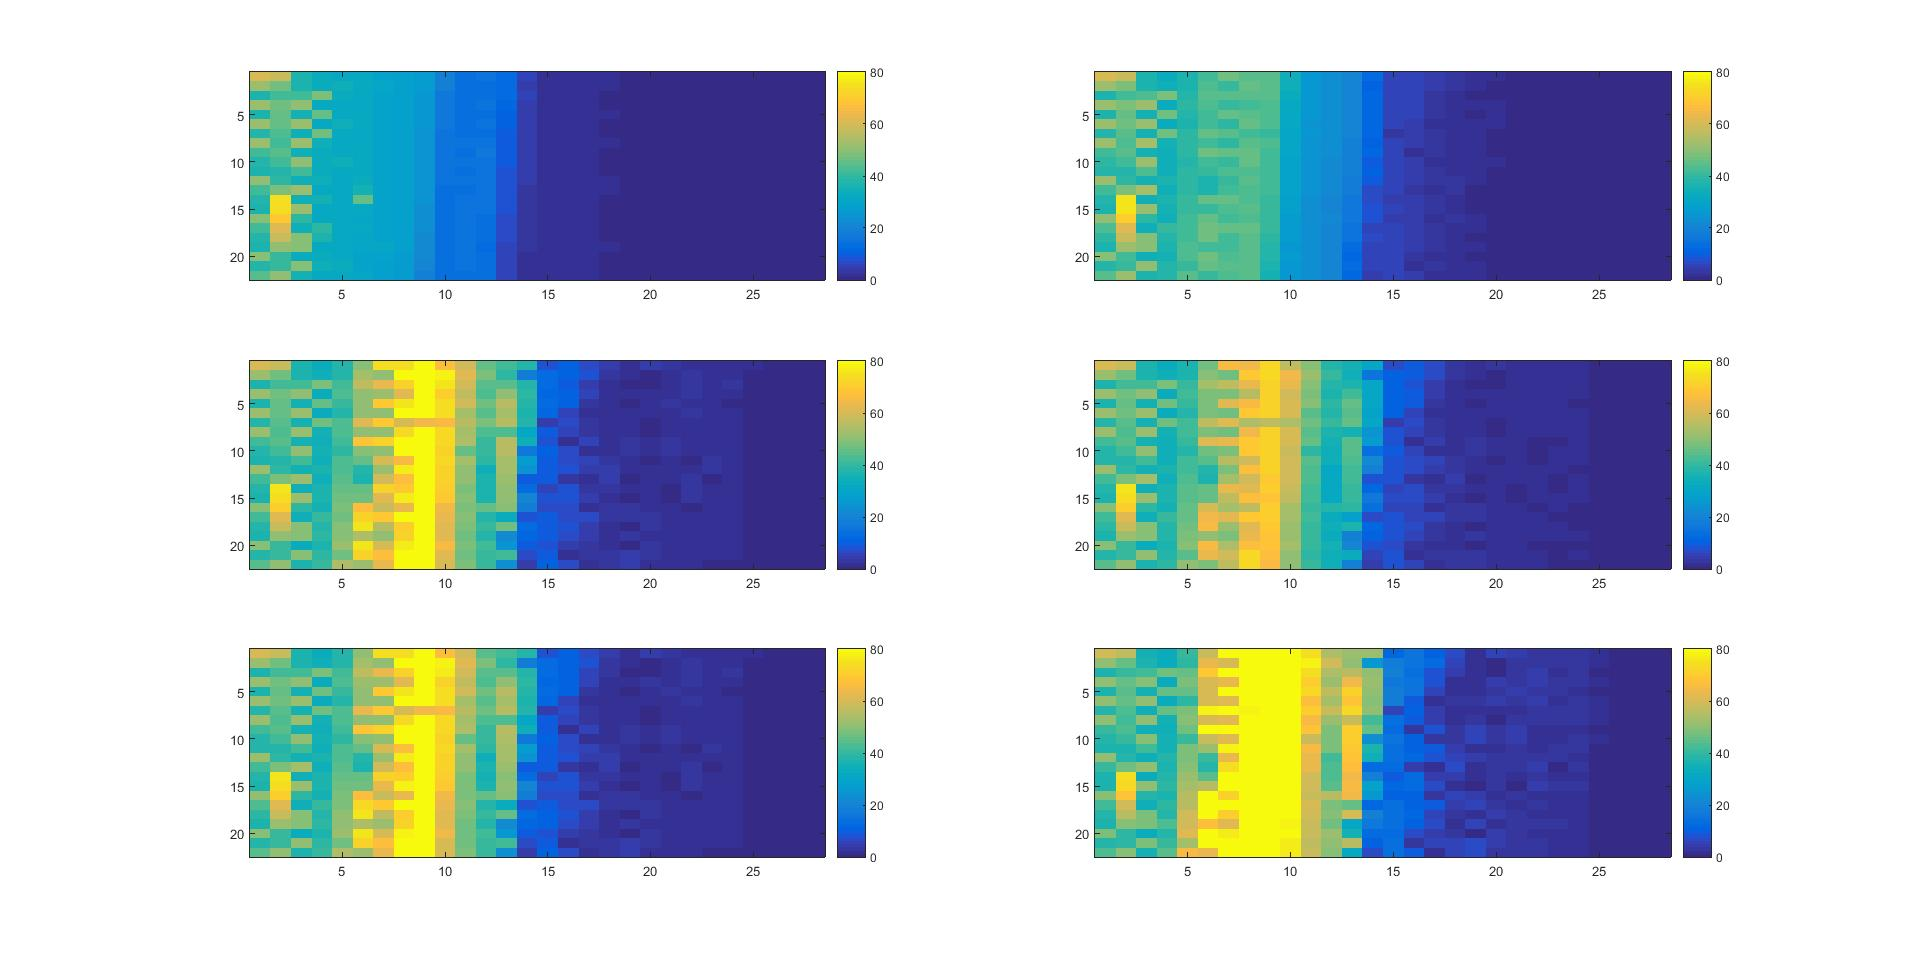
\includegraphics[width=2in]{img/pc_fea_mean/PC8.jpg}}
  \caption{ PC重构敏感性 }
\end{figure}
\end{frame}

\begin{frame}{重构结果----各PC在重构中给定权重不同时的结果}
\begin{figure}
  \centering
  \subfigure[PC 9]{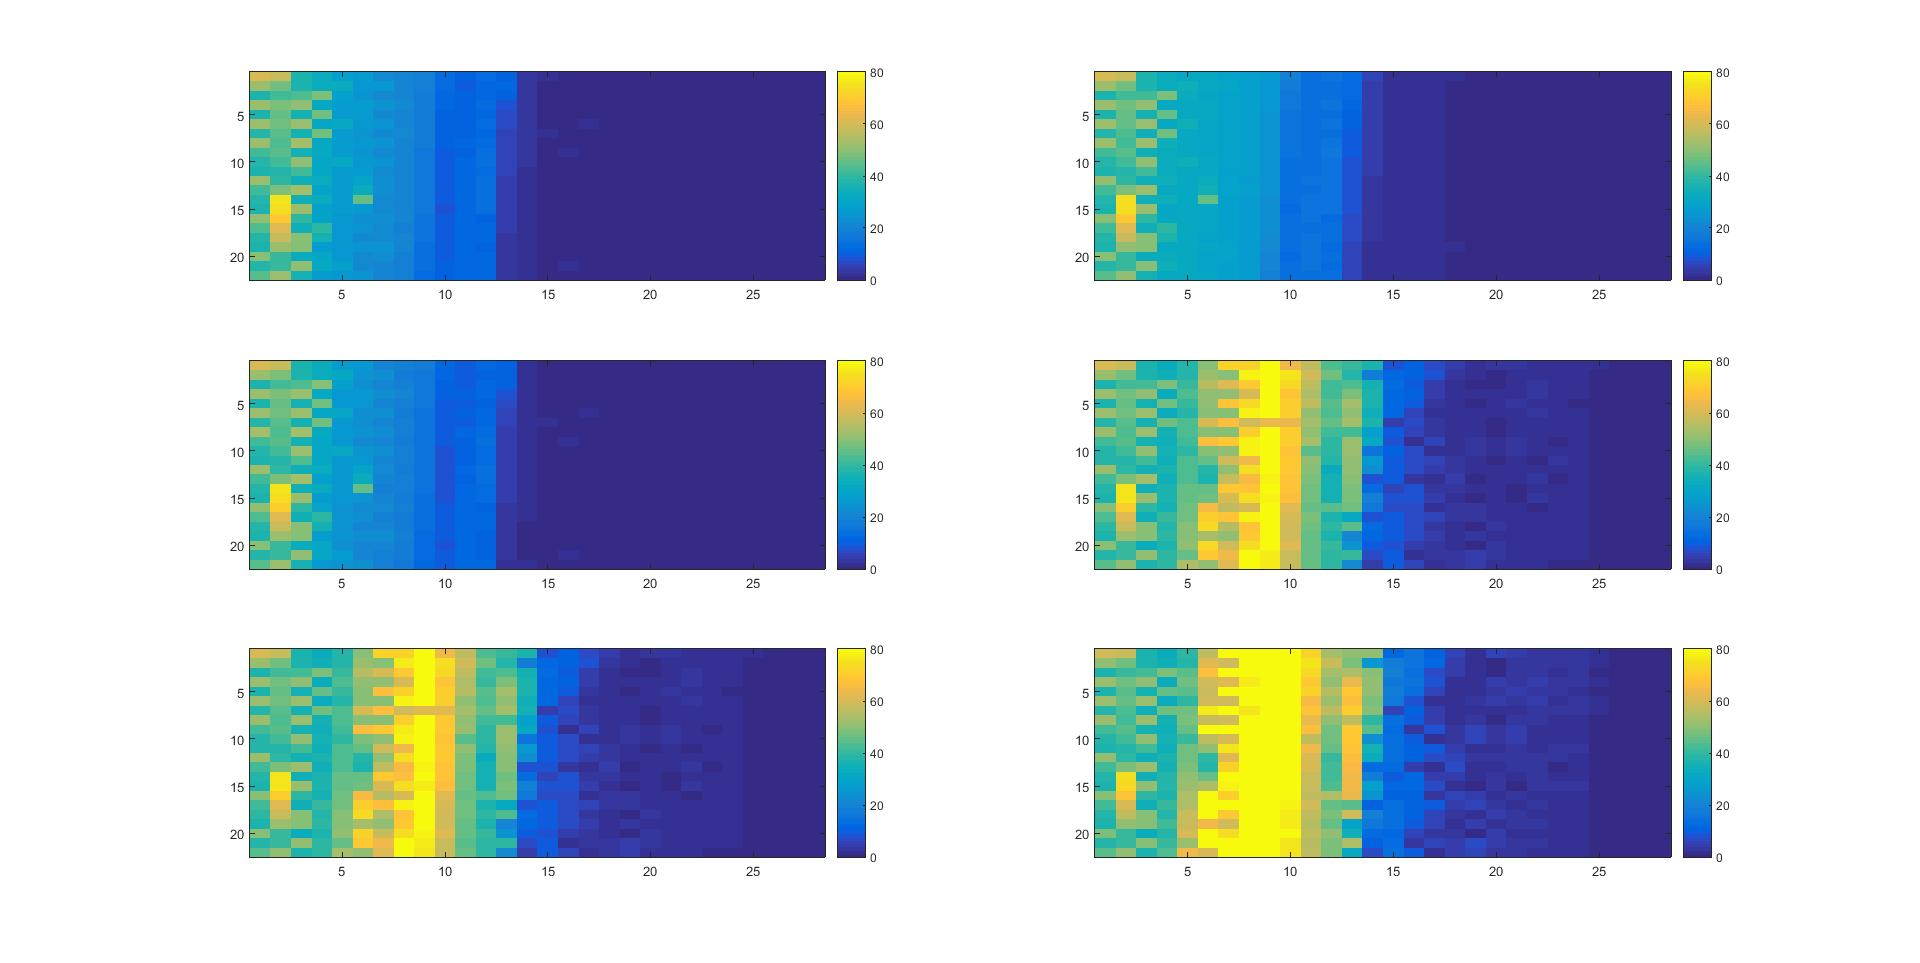
\includegraphics[width=2in]{img/pc_fea_mean/PC9.jpg}}
  \subfigure[PC 10]{\includegraphics[width=2in]{img/pc_fea_mean/PC10.jpg}}
  \caption{ PC重构敏感性 }
\end{figure}
可以看到:对不同权重修改后,重构结果差异大的地方所在的谱带不同。得到的PC提取到了一些谱带的特征。
\end{frame}

\section{Estimation}
\begin{frame}{高光谱数据压缩评估指标}
\begin{card}
信息论:信息容量(Mutual information);信噪比(SNR);峰值信噪比(PSNR)(page73\cite{陈雨时2014})\\
压缩比(CR)(page74\cite{陈雨时2014})\\
重构正确度:MSE
\end{card}
\end{frame}

\begin{frame}{高光谱数据压缩评估指标}
\begin{card}
信息论:信息容量(Mutual information);信噪比(SNR);峰值信噪比(PSNR)(page73\cite{陈雨时2014})\\
压缩比(CR)(page74\cite{陈雨时2014})\\
重构正确度:MSE
\end{card}
\end{frame}



\begin{frame}{高光谱数据压缩评估指标——信息容量}
\begin{cardTiny}[可参考第六章\cite{2014数学之美}]
\begin{equation}
I=H\left(X\right)-H\left(X|Y\right)
\end{equation}
$H\left(X\right)=-\sum\limits_{x\in X}p\left(x\right)\log p\left(x\right)$为信息熵。
特别的,当$连续信源X \sim \mathcal{N} \left( \mu,\Sigma \right)$时,$H\left(X\right)=\frac{1}{2}\ln \left| \Sigma \right|{\color{green}+\frac{1}{2}\ln 2\pi}$(??我推导的与\cite{杜华栋2010}公式2相比差常数项,请自行验证,如果推导错误请帮我纠错)。
\begin{equation}
I=\frac{1}{2}\log \Sigma_x-\frac{1}{2}\log \Sigma_{X|Y}
\end{equation}
同化中,
\begin{equation}
I=\frac{1}{2}\log \left|B\right|-\frac{1}{2}\log \left|\Sigma_{X^a|\mathcal{Y}}\right|
\end{equation}
{\color{primary}度量加入观测后,分析场的不确定性被减少了多少。}注意,上式第二项的方差不是3DVAR公式中的R。
\end{cardTiny}
\end{frame}

\begin{frame}{高光谱数据压缩评估指标}
\begin{card}[$\Sigma_{X^a|\mathcal{Y}}$估算\cite{杜华栋2010}]
{\color{green}这里公式的表述是我自己改了一下,请自行对照同化公式再验证一下。不确保我对同化公式的理解一定正确}
\begin{equation}
\Sigma_{X^a|\mathcal{Y}}=B-BK^T\left(KBK^T+R\right)^{-1}KB
\end{equation}
其中$K$为权重函数矩阵,可由RTTOV算出。
\end{card}
\end{frame}



\section{Issues}
\begin{frame}{问题}
\begin{itemize}
\item 数据集的选取:有云无云?台风与一般天气?海上陆地??
\item 权重函数矩阵的计算:RTTOV?
\item 分波段分析:数据集标注?
\end{itemize}
%\end{card}
\end{frame}



%\begin{frame}{tiny card}
%\begin{cardTiny}
%
%\end{cardTiny}
%
%\begin{card}
%{\color{primary} \textbackslash begin\{cardTiny\}\\[2mm]}
%\null\qquad \textit{[your content here]}\\[2mm]
%{\color{primary} \textbackslash end\{cardTiny\}}
%\end{card}
%\begin{card}
%Tiny card is useful for labels where too much whitespace gets in the way. 
%\end{card}
%\end{frame}

%\begin{frame}{Cards can be filled with anything you want}
%
%\begin{card}
%\centering$V(x) = \left\{ y \in \mathbb{R}^n \,|\, \forall z \in P, z\neq x:\, \|y-x\|\leq\|y-z\| \right\}$
%\end{card}
%
%\begin{card}
%\centering
%\begin{tabular}{lcr}
%left & center & right \\
%\hline
%1 & 2 & 3 \\
%\end{tabular}
%\end{card}
%
%\begin{card}
%\begin{theorem}[Pythagorean]
%The sum of the areas of the two squares on the legs equals the area of the square on the hypotenuse.
%\end{theorem}
%\end{card}
%\end{frame}
%
%\begin{frameImg}{img/rudolfinum.jpg}
%\vspace*{60mm}
%\begin{cardTiny}
%Lastly it is possible to set image as a background for a frame:\\[2mm]
%{\color{primary} \textbackslash begin\{frameImg\}["height"]\{file name\}\\[2mm]}
%\null\qquad \textit{[your content here]}\\[2mm]
%{\color{primary} \textbackslash end\{frameImg\}}
%\end{cardTiny}
%\end{frameImg}
%
%\begin{frameImg}[height]{img/rudolfinum.jpg}
%\vspace*{60mm}
%\begin{cardTiny}
%Parameter {\color{primary} ["height"]} determines the dimension that is stretched to cover the frame ({\color{primary} ["width"]} is default).
%\end{cardTiny}
%\end{frameImg}
%
%\begin{frame}
%\begin{card}
%Feel free to submit any issues you find on github: \\
%{\footnotesize \url{https://github.com/edasubert/beamerMaterialDesign}}
%\end{card}
%\end{frame}
% 注意一定要在文中引用才不会出错(至少引用一个)
\begin{frame}{参考文献}
\bibliographystyle{plain}
\bibliography{bib/comp}
\end{frame}
\end{document}
